\documentclass[10pt,landscape]{scrartcl}

\usepackage[english]{babel}
% \usepackage[ngerman]{babel}
\usepackage[utf8]{inputenc}

\usepackage{lmodern}

\usepackage{ifthen}

\usepackage{graphicx}
% \usepackage{pstricks}
% \usepackage{relsize}
% \usepackage[decimalsymbol=comma,exponent-product = \cdot, per=frac]{siunitx}
% \sisetup{range-phrase=\,bis\,}

\usepackage{xargs}
\usepackage{calc}
\usepackage{amsmath}
\usepackage{amsfonts}
\usepackage{mathtools}
\usepackage{amssymb}

\usepackage{cancel}
\usepackage{trfsigns}
\usepackage{array}
\usepackage{enumerate}
\usepackage{enumitem}

\usepackage{caption}
\usepackage{subcaption}

\usepackage{multicol}

\usepackage{pdflscape}
\usepackage[table]{xcolor}

\usepackage{float}

%%%%%%%%%%%%%%%%%%%%%%%%%%%%%%%%%%%%%%%%%%%%%%%%%%%%%%%%%%%%%%%%%%%%%%%%%%%%%%%%
\newboolean{WITHPSTRICKS}
\setboolean{WITHPSTRICKS}{false}


\newcommand{\PROFESSOR}{Prof.\ Dr.\ Thomas Carraro}
\newcommand{\ASSISTANT}{\setlength{\tabcolsep}{0pt}\begin{tabular}{l} Dr. Ulrike Kochan-Eilers\end{tabular}}

\newcommand{\Jahr}{2025}
% \newcommand{\Trimester}{HT}
\newcommand{\Trimester}{WT}
\newcommand{\Kurs}{Mathematik II/B (WI/ET)}
\newcommand{\TYPE}{Aufgabenblatt}
\newcommand{\BLATT}{0}
\newcommand{\TOPIC}{Zusatzblatt zur Vorbereitung auf Bonusklausur}

%%%%%%%%%%%%%%%%%%%%%%%%%%%%%%%%%%%%%%%%%%%%%%%%%%%%%%%%%%%%%%%%%%%%%%%%%%%%%%%%
\newboolean{mitLoes}
\setboolean{mitLoes}{false}
\setboolean{mitLoes}{true}

%%%%%%%%%%%%%%%%%%%%%%%%%%%%%%%%%%%%%%%%%%%%%%%%%%%%%%%%%%%%%%%%%%%%%%%%%%%%%%%%

%\setboolean{WITHPSTRICKS}{false}
\setboolean{WITHPSTRICKS}{true}

\usepackage{pgfplots}
\pgfplotsset{compat=1.18}


\usepackage{tikz}
\usetikzlibrary{arrows,automata,backgrounds,calendar,decorations.pathmorphing,fadings,shadings,calc,intersections}
\usetikzlibrary{decorations.pathreplacing}
\usetikzlibrary{decorations.shapes}
\usetikzlibrary{decorations.footprints}
\usetikzlibrary{decorations.text}
\usetikzlibrary{positioning}
\usetikzlibrary{through}
\usepackage[utf8]{inputenc}


\ifthenelse{\boolean{WITHPSTRICKS}}{%
\usepackage{auto-pst-pdf}
\usepackage{pstricks,pst-plot,pst-text}
}{}

\usepackage{pgfplots}

%%%%%%%%%%%%%%%%%%%%%%%%%%%%%%%%%%%%%%%%%%%%%%%%%%%%%%%%%%%%%%%%%%%%%%%%%%%%%%%%
\usepackage{mbdefAufgaben}

%%%%%%%%%%%%%%%%%%%%%%%%%%%%%%%%%%%%%%%%%%%%%%%%%%%%%%%%%%%%%%%%%%%%%%%%%%%%%%%%
\newboolean{mitErg}
%\setboolean{mitErg}{false}

%%%%%%%%%%%%%%%%%%%%%%%%%%%%%%%%%%%%%%%%%%%%%%%%%%%%%%%%%%%%%%%%%%%%%%%%%%%%%%%%
\newcounter{Aufg}
\setcounter{Aufg}{0}
\newcounter{Blatt}
\setcounter{Blatt}{1}

%%%%%%%%%%%%%%%%%%%%%%%%%%%%%%%%%%%%%%%%%%%%%%%%%%%%%%%%%%%%%%%%%%%%%%%%%%%%%%%%
%\usepackage{KopfEnglish}

% Seitenraender
%\textwidth = 285mm
%\textheight = 180mm
%\leftmargin 5mm
%\oddsidemargin = -20mm
%\evensidemargin = -20mm
%\topmargin = -25mm
%\parindent 0cm
%\columnsep 2cm

% % % Aufgabenstellung
% % % Schwierungkeitsgrad mit "e" , "f" oder "v" angeben
% % % "e" Einführung   
% % % "f" Festigung
% % % "v" Vertiefung  

\newcommand{\Aufgabe}[3][]{
\stepcounter{Aufg}
\subsubsection*{Aufgabe 
\arabic{Aufg}\ifthenelse{\equal{#1}{e}}{}{\ifthenelse{\equal{#1}{f}}{
$\!\!{}^\star$}{\ifthenelse{\equal{#1}{v}}{$^{\star\star}$}{}}}{: #2}}
{#3}
}
% % % Ergebnisse jeweils am Ende des Aufgabenblattes Anzeigen
\newcommand{\Ergebnisse}{}
\makeatletter
\newcommand{\Ergebnis}[1]{
	\g@addto@macro{\Ergebnisse}{#1}
}
\makeatother
\makeatletter
\newcommand{\ErgebnisC}[2]{
\@ifundefined{c@#1}
{\newcounter{#1}}
{}
\setcounter{#1}{\theAufg}

\ifthenelse{\boolean{mitErg}}{	\g@addto@macro{\Ergebnisse}{\subsubsection*{Ergebnisse zu Aufgabe \arabic{#1}:}
}%
	\g@addto@macro{\Ergebnisse}{#2}}{}
}
\makeatother


% % % Lösungen
\newcommand{\Loesung}[1]{
	\ifthenelse{\boolean{mitLoes}}
	{\subsubsection*{Lösung \arabic{Aufg}:}
		#1}
	{}
}
% % % % % % % % % % % % % % % % % % % % % % % % % % % % % % % % % % % % % % % % % % % % % % % % % % % % % %
% % % % % % % % % % % % % % % % % % % % % % % % % % % % % % % % % % % % % % % % % % % % % % % % % % % % % %
% % % % % % % % % % % % % % % % % % % % % % % % % % % % % % % % % % % % % % % % % % % % % % % % % % % % % %
\begin{document}
%\begin{twocolumn}
% % % % % % % % % % % % % % % % % % % % % % % % % % %

%%%%%%%%%%%%%%%%%%%%%%%%%%%%%%%%%%%%%%%%%%%%%%%%%%%%%%%%%%%%%%%%%%%%%%%%%%%%%%%%
% Set the TITLE of the sheet here:
%\uebheader{\Kurs}{\arabic{Blatt}}{\Trimester\,\Jahr}{\TOPIC}
%\uebheader{\Kurs}{\arabic{Blatt}}{\Trimester\,\Jahr}{\TOPIC}
%\uebheader{\Kurs}{\arabic{Blatt}}{\Trimester\,\Jahr}{\TOPIC}
%\ruleBig

\setboolean{mitErg}{false}
%\setboolean{mitErg}{true}


%%%%%%%%%%%%%%%%%%%%%%%%%%%%%%%%%%%%%%%%%%%%%%%%%%%%%%%%%%%%%%%%%%%%%%%%%%%%%%%%
% Set the INTRODUCTION section of the sheet here:
% \input{introduction.tex}

\textbf{Einführende Bemerkungen}

\begin{itemize}
\item Vermeiden Sie die Verwendung von Taschenrechnern oder Online-Ressourcen.
\end{itemize}

\ruleBig
\Aufgabe[e]{Partielle Ableitungen}{
Bestimmen Sie die ersten partiellen Ableitungen der folgenden reellen Funktionen und geben Sie diese Ableitungen in Matrixschreibweise an: 
\[
\begin{array}{rclcrcl}
\mathbf{i)} &  & f(x,y)=\, e^{xy^3} & \;\;\;\;\; & \mathbf{ii)} & & g(x,y)=\sin(x^2-y) \\ 
&  &  &  &  &  &  \\ 
\mathbf{iii)} &  & h(x,y)=(2x-y)^2 +\ln(xy) &  & \mathbf{iv)} &  & p(x,y)=\ln(x+y^2) - e^{2xy}+3x\\
&  &  &  &  &  &  \\ 
\mathbf{v)} &  & q(x,y,z)= e^{x-y}\cos(5z)
\end{array}
\]
}

\Loesung{

\begin{iii}
\item \begin{align*}
\nabla f(x,y)=&\left( y^3 e^{xy^3}\;,\;3y^2x e^{xy^3}\right)^\top\\
\end{align*}
\item \begin{align*}
\nabla g(x,y)=& \Big( 2x \cos(x^2-y)\;,\;-\cos(x^2-y)\Big)^\top \\
\end{align*}
\item \begin{align*}
\nabla h(x,y)=&\Big( 4(2x-y)+\dfrac{1}{x}\;,\;-2(2x-y) + \dfrac{1}{y}\Big)^\top\\
\end{align*}
\item \begin{align*}
\nabla p(x,y)=&\big(\dfrac{1}{x+y^2}-2ye^{2xy}+3\;,\; \dfrac{2y}{x+y^2}-2xe^{2xy}\big)^\top\\
\end{align*}
\item \begin{align*}
\nabla q(x,y,z) =&\big(e^{x-y} \cos(5z)\;,\; -e^{x-y}\cos(5z)\;,\; -5e^{x-y} \sin(5z)\big)^\top\\
\end{align*}
\end{iii}
}

% \ErgebnisC{dummy}
% {
% 
% }
\Aufgabe[e]{Richtungsableitungen} {

Gegeben seien die skalarwertige Funktion $f(x,y)$ und die vektorwertige Funktion $\vec g(x,y)$ 
$$f(x,y)=x^2y^3\qquad \text{ und } \qquad \vec g(x,y)=(x^2+y,\, xy)^\top.$$
Berechnen Sie die Richtungsableitung beider Funktionen im Punkt $\vec P = (1,\, 2)^\top$ in Richtung $\vec h:=(3,4)^\top$.

}



\Loesung{

Zun\"achst berechnen wir die die ersten Ableitungen der beiden Funktionen:
\begin{align*}
\nabla f(x,y) =& (2xy^3,\, 3x^2y^2)^\top\\
\vec J_g(x,y) &= 
\begin{pmatrix} 
2x & 1\\
y & x
\end{pmatrix}.
\end{align*}
Nun berechnen wir die ersten Ableitungen im Punkt $\vec P = (1,\, 2)^\top$:
\begin{align*}
\nabla f(1,2) =& (16,\, 12)^\top\\
\vec J_g(1,2) &= 
\begin{pmatrix} 
2 & 1\\
2 & 1
\end{pmatrix}.
\end{align*}
Desweiteren ben\"otigen wir den Normalenvektor in Richtung $\vec h$:
$$\vec{\hat h}=\frac 1{5}(3,\, 4)^\top$$
Damit ergeben sich dann die Richtungsableitungen:
\begin{align*}
\frac{\partial f}{\partial \vec{\hat h}}(x,y)=& \skalar{\vec{\hat h},\, \nabla f(x,y,z)}=\frac
{96}{5}\\
\frac{\partial \vec g}{\partial \vec{\hat h}}(x,y)=& \vec J_g(1,2) \cdot \vec{\hat h}
= (2,\, 2)^\top
\end{align*}

}
\Aufgabe[e]{Taylor--Entwicklung in 2 Dim.}{
Gegeben sei \ $f:\R^2 \to \R$  \ mit \ $f(x,y)=e^{x}\sin(y)$.
Bestimmen Sie das Taylorpolynom 2. Grades von \ $f$ \ für den Entwicklungspunkt \ $(0,0)$\,.
}

\Loesung{
 Mit den partiellen Ableitungen 
  \[
  \begin{array}{rclcl}
  f_x & = & e^{x}\sin(y) & \Rightarrow  & f_x(0,0)=0\ , \\
  f_y & = & e^{x}\cos(y) & \Rightarrow  & f_y(0,0)=1\ , \\
  f_{xx} & = & e^{x}\sin(y)& \Rightarrow  & f_{xx}(0,0)=0\ , \\
  f_{xy} & = & e^{x}\cos(y) & \Rightarrow  & f_{xy}(0,0)=1\ , \\
  f_{yy} & = & -e^{x}\sin(y) & \Rightarrow  & f_{yy}(0,0)=0
  \end{array}
\]
folgt
\begin{align*}
T_{f,2}(x,y)\  = & \  f(0,0) + f_x(0,0)(x-0)+f_y(0,0)(y-0)+ \frac{1}{2} f_{xx}(0,0)(x-0)^2 \\
+ & \frac{1}{2}f_{yy}(y-0)^2  +f_{xy}(0,0)(x-0)(y-0) \\
 = & \  y+xy
\end{align*}

}

% \ErgebnisC{dummy}
% {
% 
% }


\Aufgabe[]{Newton-Verfahren }{
Gegeben sei die Funktion $f:\R ^3\rightarrow \R $ durch 
$$f(x,y)=x^3-3xy^2.$$
Gesucht sind die station\"aren Punkte dieser Funktion. 
\begin{abc}
\item Geben Sie an, welche Bedingung ein station\"arer Punkt $\vec x\in\R^3$ erf\"ullen muss. 
\item Um eine N\"aherung f\"ur einen solchen Punkt zu berechnen, soll das dreidimensionale Newton-Verfahren angewendet werden. Auf welche Funktion wird das Newton-Verfahren angewendet?\\
Geben Sie die Iterationsvorschrift an. 
\item F\"uhren Sie f\"ur den Startvektor $\vec x_0=\begin{pmatrix}1\\1\end{pmatrix}$ einen Iterationsschritt durch. 
\item Geben Sie ein geeignetes Abbruchkriterium des Newton-Verfahrens an. (Dieses Kriteriums ist \textbf{nicht} auszuwerten.)
\end{abc}
}

\Loesung{
\begin{abc}
\item In einem station\"aren Punkt muss der Gradient der Funktion $f$ verschwinden: 
$$\vec 0\overset != \nabla f(x,y,z)=\begin{pmatrix}
3x^2-3y^2\\
-6xy
\end{pmatrix}$$

\item Das Newton-Verfahren wird auf die Funktion $\vec F(x,y,z)=\nabla f(x,y,z)$ angewendet. Die Ableitung dieser Funktion ist
\begin{align*}
&\vec F'(x,y,z)\Bigl(=H_f(x,y,z)\Bigr)\\
=&\begin{pmatrix}
6x &  -6y\\
-6y & -6x 
\end{pmatrix}.
\end{align*}
Zu gegebenem Startwert $\vec x_0$ wird die folgende Iteration durchgef\"uhrt: \\
F\"ur $j=0,1,2,\hdots$: 

\begin{iii}
\item L\"ose das lineare Gleichungssystem $\vec F'(\vec x_j)\Delta \vec x = -\vec F(\vec x_j)$ nach $\Delta \vec x$ auf.
\item Berechne n\"achste Iteration $\vec x_{j+1}=\vec x_j+\Delta \vec x$. 
\end{iii}

\item F\"ur den gegebenen Startvektor $\vec x_0=\left(1,1\right)^\top$ ergibt sich 
zun\"achst 
$$\vec F\left(1,1\right)=\begin{pmatrix}0 \\-6 \end{pmatrix}\text{ und }\vec F'\left(1,1\right)=\begin{pmatrix}
 6& -6 \\
-6 & -6\end{pmatrix}.$$
Die L\"osung des Gleichungssystems $\vec F'(\vec x_0) \Delta \vec x = -\vec F(\vec x_0)$ 
ergibt
$$\Delta \vec x= \begin{pmatrix}-\frac{1}{2}\\-\frac{1}{2} \end{pmatrix}$$
und als n\"achsten Iterationsschritt
$$\vec x_1=\vec x_0+\Delta \vec x = \begin{pmatrix}\frac{1}{2}\\\frac{1}{2} \end{pmatrix}.$$

\item Geeignete Abbruchkriterien sind etwa
$\Vert{\vec F(\vec x_k)}\Vert<\varepsilon$ oder $\Vert{\vec x_k-\vec x_{k-1}}\Vert<\varepsilon$ mit fest vorgegebenem $\varepsilon>0$. \\
Desweiteren empfiehlt es sich, die Iteration nach $N$ Schritten (z. B. $N=1000$) abzubrechen, auch wenn das Abbruchkriterium nicht erf\"ullt ist.  
\end{abc}
}
\Aufgabe{Stationäre Punkte}{
Gegeben sei die Funktion:

$$
f(x,y) = x^3+axy+y^3 \quad \text{ mit } \quad a \in \mathbb{R}.
$$

\begin{abc}
	\item
	Bestimmen Sie alle stationären Punkte in Abhängigkeit von $a$.
	\item
	Klassifizieren Sie diese für $a\neq 0$ als Minimum, Maximum oder Sattelpunkt.
\end{abc}
\ifthenelse{\boolean{mitLoes}}


}
\Loesung{
\begin{abc}
	
	\item
	Der Gradient ist gegeben durch:
	\[
	\nabla f(x, y) = \left( 3x^2+ay, ax+3y^2 \right)
	\]
	
	Um die stationären Punkte zu finden, setzen wir den Gradienten gleich 0:
	
	1. $3x^2+ay = 0$

	2.  $ax+3y^2 = 0$ \\
	
F\"ur den Fall $a=0$ erhalten wir $3x^2 =0$ und $3y^2=0$, d.h. einen station\"aren Punkt bei (0,0).
F\"ur $a \neq 0$ lösen wir die erste Gleichung nach $y$ auf:
\begin{align*}
	&3x^2+ay = 0 \quad \Rightarrow \quad y = -\dfrac{3x^2}{a}.
\end{align*}
Einsetzen in die zweite Gleichung ergibt:
\begin{align*}
ax+3y^2 &= 0 \\
ax+3( -\dfrac{3x^2}{a})^2 &= 0 \\
ax + \frac{27}{a^2} x^4 &= 0 \\
x(a+ \frac{27}{a^2} x^3) &= 0
\end{align*}
Daraus ergeben sich die stationären Punkte $(0,0)$ und $(-\frac{1}{3},-\frac{1}{3})$.

	\item
	Für $a \neq 0$ ist die Hesse-Matrix gegeben als:
	$$
		\boldsymbol H(x,y) =
		\begin{pmatrix}
				6x & a  \\
				a & 6y
			\end{pmatrix}
		$$
		
\begin{itemize}
			
\item Ausgewertet in $(0,0)$ erhalten wir:
				$$
				\boldsymbol H\left(0,0\right) = \begin{pmatrix}
					0 & a \\
					a & 0
				\end{pmatrix}
				$$
Für die Determinante ergibt sich $det(\boldsymbol H\left(0,0\right)) = -a^2 <0$. Daher ist die Matrix indefinit und der Punkt $(0,0)$ ist ein Sattelpunkt.

\item  Ausgewertet in $(-\frac{1}{3},-\frac{1}{3})$ erhalten wir:
$$
\boldsymbol H\left(-\frac{1}{3},-\frac{1}{3}\right) = \begin{pmatrix}
	-2a & a \\
	a & -2a
\end{pmatrix}
$$
Für die Determinante ergibt sich $det(\boldsymbol H\left(-\frac{1}{3},-\frac{1}{3}\right)) = 3a^2 >0$. Damit erhalten wir für $a<0$ ein lokales Minimum und für $a>0$ ein lokales Maximum.
\end{itemize}
	
	
\end{abc}

}

\Aufgabe[e]{Integration}{
\begin{abc}
\item Berechnen Sie folgende Integrale
\begin{align*}
I_1=& \int x^2 \ln(x)\mathrm{d} x,\\
I_2=& \int \frac{x}{(x^2+1)^2} \mathrm{d} x,\\
I_3=& \int \frac{3x+2}{x^2+6x+9}\mathrm{d} x.
\end{align*}
\vspace*{-0.25cm}

\item Berechnen Sie das Integral
$$
I = \int_G y\ \mathrm{d} x \mathrm{d} y
$$
wobei $G\subset \mathbb R^2$ der Bereich ist, der zwischen den beiden Graphen der folgenden Funktionen liegt
$$
y = x^2 \quad \text{und} \quad y=2x.
$$
\end{abc}
}

\Loesung{
\begin{abc}
\item 
Das erste Integral ergibt sich durch einmalige partielle Integration: 
\begin{align*}
I_1=&  \int x^2 \ln{x}\mathrm{d} x\\
=& \frac{1}{3}x^3 \ln(x) - \frac{1}{3} \int x^3 \frac{1}{x} \mathrm{d} x\\
=& \frac{1}{3} x^3\ln{x} - \frac{1}{3} \int x^2 \mathrm{d} x\\
=& \frac{1}{3} x^3\ln{x} - \frac{1}{9} x^3 + c.
\end{align*}

F\"ur das zweite Integral ergibt die Substitution $u=x^2+1$, $\mathrm{d} u = 2x\mathrm{d} x$
\begin{align*}
	I_2=& \int \frac{1}{2} \frac{1}{u^2}\mathrm{d} x\\
	=& \frac{1}{2} (-1) \frac{1}{u} +c\\
	=& -\frac{1}{2} \frac{1}{u} + c \\
	=& -\frac{1}{2} \frac{1}{x^2+1} +c.
\end{align*}

Das dritte Integral ergibt sich durch die Partialbruchzerlegung: 
\begin{align*}
I_3=\int \frac{3x+2}{(x+3)^2}\mathrm{d} x
= \int\frac{3x+2}{(x+3)(x+3)}\mathrm{d} x\\
\end{align*}
\begin{align*}
\frac{3x+2}{(x+3)(x+3)} =& \frac{A}{x+3} + \frac{B}{(x+3)^2}\quad || \cdot (x+3)(x+3) \\
	\Longleftrightarrow 3x+2 =& A(x+3) + B \\
	 -7 =& B  \quad \Longrightarrow B = -7 \\
	 2=& 3A-7 \quad \Longrightarrow A = 3
\end{align*}
\begin{align*}
I_3=&\int\left(\frac{3}{(x+3)} - \frac{7}{(x+3)^2}\right)\mathrm{d} x\\
	 = &  3\ln{(|x+3|)} + \frac{7}{x+3} + c
 \end{align*} 
 
\item 
Die Fläche zwischen den beiden Graphen kann als Normalenbereich bezüglich x formuliert werden
$$
G := \{(x,y)\in \mathbb R^2: 0 \le x \leq 2\ \land\ x^2 \leq y \leq 2x \}
$$


\begin{align*}
I &= \int_G y\ \mathrm{d} x \mathrm{d} y,\\
&=\int_{x=0}^2 \int_{y=x^2}^{2x} y\ \mathrm{d} y \mathrm{d} x,\\
&=\int_0^2 \frac{1}{2}[y^2]_{x^2}^{2x}  \mathrm{d} y,\\
&= \frac{1}{2} \int_0^2 4x^2-x^4 \mathrm{d} y,\\
&= \frac{1}{2} \left[ \frac{4}{3} x^3 - \frac{1}{5}x^5 \right]_0^2 \\
&= \frac{1}{2} \left[ \frac{4}{3} 8 - \frac{1}{5} 32 \right] \\
&= \frac{1}{2} \frac{64}{15} \\
&= \frac{32}{15}
\end{align*}
\end{abc}

\begin{center}
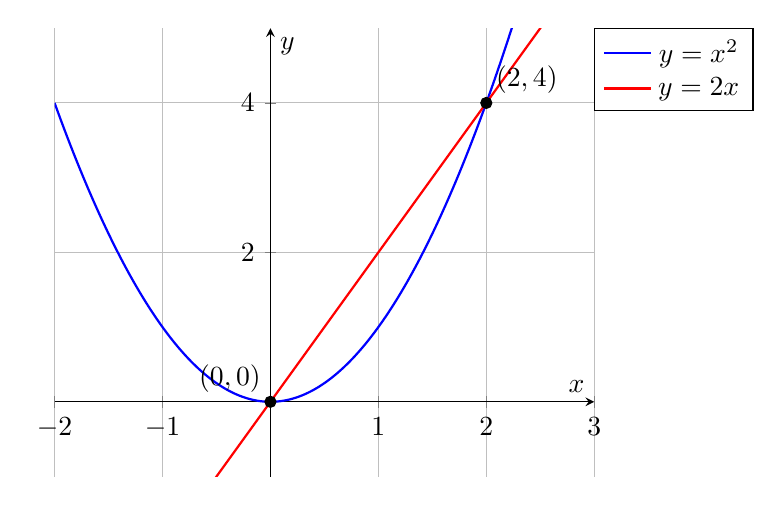
\begin{tikzpicture}
  \begin{axis}[
    axis lines = center,
    xlabel = $x$,
    ylabel = $y$,
    grid = both,
    legend style={at={(1,1)}, anchor=north west},
    xmin=-2, xmax=3,
    ymin=-1, ymax=5,
    samples=200
  ]
    % Funktionen
    \addplot[domain=-2:3, thick, blue]{x^2};
    \addlegendentry{$y = x^2$}

    \addplot[domain=-2:3, thick, red]{2*x};
    \addlegendentry{$y = 2x$}

    % Schnittpunkte
    \addplot[only marks, mark=*, mark size=2pt] coordinates {(0,0) (2,4)};
    \node[anchor=south east] at (axis cs:0,0) {$(0,0)$};
    \node[anchor=south west] at (axis cs:2,4) {$(2,4)$};

  \end{axis}
\end{tikzpicture}
\end{center}
}

% 



%%%%%%%%%%%%%%%%%%%%%%%%%%%%%%%%%%%%%%%%%%%%%%%%%%%%%%%%%%%%%%%%%%%%%%%%%%%%%%%%


%%%%%%%%%%%%%%%%%%%%%%%%%%%%%%%%%%%%%%%%%%%%%%%%%%%%%%%%%%%%%%%%%%%%%%%%%%%%%%%%
\end{twocolumn}

\end{document}

%%%%%%%%%%%%%%%%%%%%%%%%%%%%%%%%%%%%%%%%%%%%%%%%%%%%%%%%%%%%%%%%%%%%%%%%%%%%%%%%
